\subsection{Forward stepwise selection}

The first method applied is the forward stepwise selection. In particular, the algorithm variant employed uses the \textit{p-value} as entrance criterion and the \textit{akaike information criterion} (AIC) as comparison metric between models. The model obtained is shown in \Tab~\ref{table:ForwardModelSummary}.

As expected, ``MIN'' and ``FTM'' are included, which resulted to be important from the preliminary analysis as well. However, there are three variables that are not significantly different from 0, with a p-value threshold of $5\%$.

\textbf{Bootstrap statistical inference}

On the obtained model we used the Bootstrap technique in order to perform statistical inference on the model coefficients. In \Tab~\ref{table:ForwardModelSummary} it is possible to see the results, that are coherent with the previous ones. This also shows that the gaussian approximation for the error is valid in this case. 

\begin{center}
	\labelText{\texttt{final\_step\_forward <- ols\_step\_forward\_p(model = f\_lm\_all)}}{mod:lrf2}
\end{center}

\begin{table}[H]
	\centering
	\begin{tabular}{|| l | r | r ||} 
		\hline
		Variable & Coefficient & p-value \\
		\hline
		intercept & -3.6316 & 0.0010 \\
		MIN & 0.2438 & 0.0000 \\
		FTM & 1.7241 & 0.0000 \\
		3P MADE & 0.2718 & 0.5840 \\
		FG\% & 0.0637 & 0.0000 \\
		TOV & 1.5675 & 0.0000 \\
		AST & -0.3606 & 0.0010 \\
		DREB & -0.2564 & 0.0010 \\
		3P\% & 0.0104 & 0.0000 \\
		OREB & 0.2878 & 0.0070 \\
		STL & -0.3920 & 0.0110 \\
		3PA & 0.3563 & 0.0550 \\
		BLK & -0.1817 & 0.0920 \\
		GP & -0.0039 & 0.0930 \\
		\hline
	\end{tabular}
	\caption{Estimated coefficients' value and corresponding p-value obtained applying forward stepwise selection to a linear regression model, given by \Mod~\ref{mod:lrf2}.}
	\label{table:BootForwardModel}
\end{table}

\vspace{0.2cm}
\noindent
\textbf{Final forward model}

The final forward model, shown in \Tab~\ref{table:ForwardFinalModelSummary}, is obtained removing the non significant variables. Instead, in \Fig~\ref{fig:ForwardFinalModelResiduals} and \Fig~\ref{fig:ForwardFinalModelResidualsDist} it is possible to see the plots of the residuals, that have a gaussian shape with 0 mean. This means that the model is likely adequate for our purposes.

\begin{center}
	\labelText{
			\texttt{forward\_lm\_fit <- update(final\_step\_forward, $\sim$.-x3p\_made-gp- blk)}
		}{mod:lrf3}
\end{center}

\begin{table}[H]
	\centering
	\begin{tabular}{|| l | r | r ||} 
		\hline
		Variable & Coefficient & p-value \\
		\hline
		intercept & -3.7388 & $<$ 0.0001 \\
		MIN & 0.2387 & $<$ 0.0001 \\
		FTM & 1.7242 & $<$ 0.0001 \\
		TOV & 1.5457 & $<$ 0.0001 \\
		AST & -0.3487 & $<$ 0.0001 \\
		FG\% & 0.0625 & $<$ 0.0001 \\
		DREB & -0.2890 & $<$ 0.0001 \\
		3P\% & 0.0107 & $<$ 0.0001 \\
		OREB & 0.2875 & 0.0024 \\
		STL & -0.3965 & 0.0051 \\
		3PA & 0.4677 & $<$ 0.0001 \\
		\hline
	\end{tabular}
	\caption{Estimated coefficients' value and corresponding p-value obtained applying forward stepwise selection to a linear regression model, given by \Mod~\ref{mod:lrf3}.}
	\label{table:ForwardFinalModelSummary}
\end{table}

\begin{figure}[H]
	\centering
	\begin{subfigure}{.5\textwidth}
		\centering
		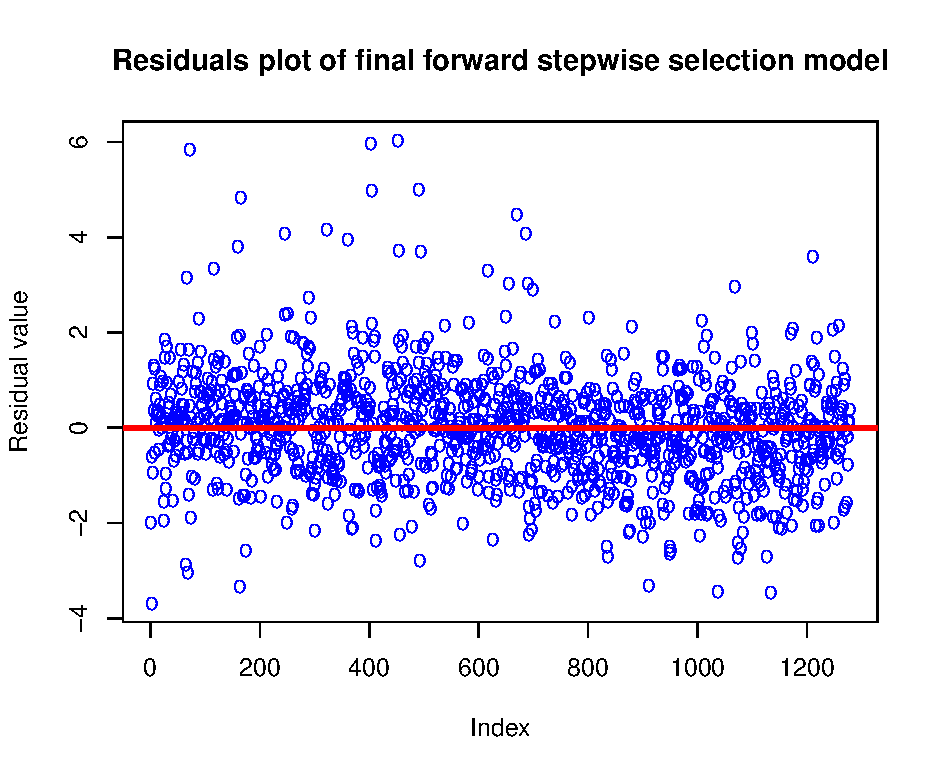
\includegraphics[width=0.7\linewidth]{ImageFiles/Regression/Forward/ForwardFinalModelResiduals.pdf}
		\caption{}
		\label{fig:ForwardFinalModelResiduals}
	\end{subfigure}%
	\begin{subfigure}{.5\textwidth}
		\centering
		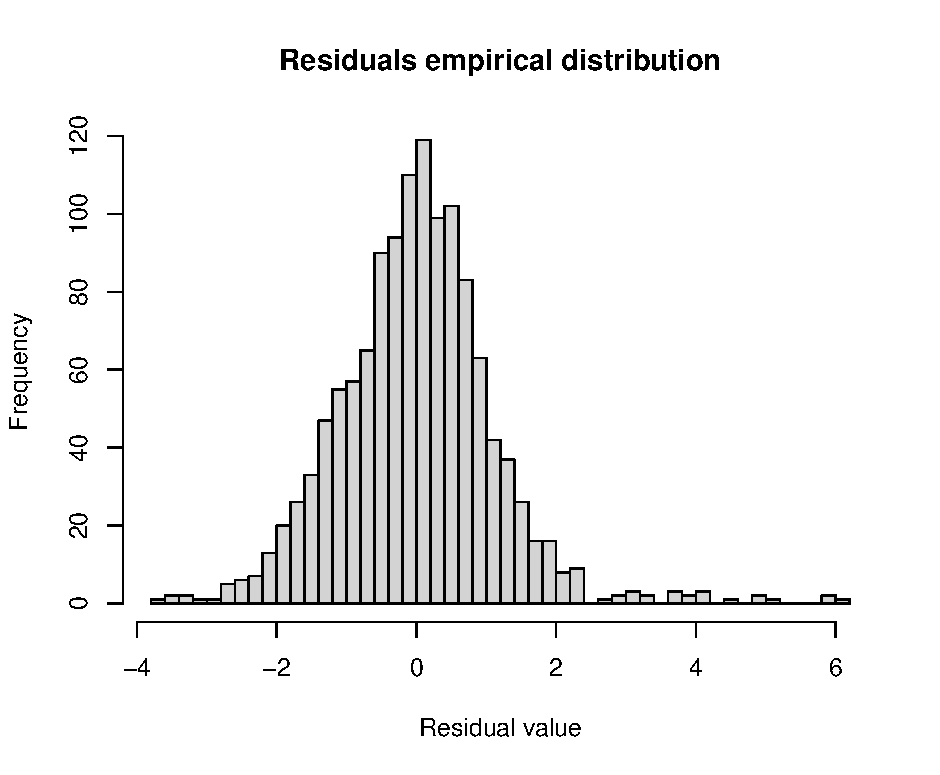
\includegraphics[width=0.7\linewidth]{ImageFiles/Regression/Forward/ForwardFinalModelResidualsDist.pdf}
		\caption{}
		\label{fig:ForwardFinalModelResidualsDist}
	\end{subfigure}
	\caption{Residuals obtained by predicting with \Mod~\ref{mod:lrf3}. (a) Plot of the residuals (mean = 0 \& var = 1.26). (b) Empirical distribution of the residuals.}
	\label{fig:FinalFSSM}
\end{figure}

